\newpage
\section{11. 盛最多水的容器}
\label{leetcode:11}

\subsection{题目}

给定 n 个非负整数 $a_{1}$,$a_{2}$,\ldots,$a_{n}$,
每个数代表坐标中的一个点 (i, $a_{i}$) 。
在坐标内画 n 条垂直线,垂直线 i 的两个端点分别为 (i, $a_{i}$) 和 (i, 0)。
找出其中的两条线,使得它们与 x 轴共同构成的容器可以容纳最多的水。

\textbf{说明}:你不能倾斜容器,且 n 的值至少为 2。

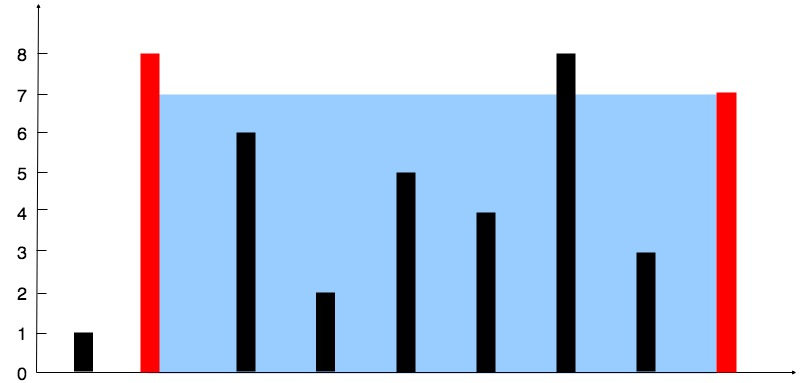
\includegraphics[width=100mm,height=50mm]{images/leetcode/question_11.jpg}

图中垂直线代表输入数组 [1,8,6,2,5,4,8,3,7]。在此情况下,
容器能够容纳水(表示为蓝色部分)的最大值为 49。

\textbf{示例}:

\begin{verbatim}
  输入: [1,8,6,2,5,4,8,3,7]
  输出: 49
\end{verbatim}

\subsection{参考题解,暴力法}

直接两重循环,遍历左右两根柱子的所有组合情况。
因为两重循环,所以时间复杂度为 O(n$^{2}$)。
因为没有而外开辟空间,所以空间复杂度为 O(1)。

\begin{verbatim}
/**
 * @param {number[]} height
 * @return {number}
 */
var maxArea = function(height) {
  let result = 0;
  for (let i = 0; i < height.length; i += 1) {
    for (let j = i + 1; j < height.length; j += 1) {
      const curWidth = j - i;
      const curHeight = Math.min(height[i], height[j]);
      const curArea = curWidth * curHeight;
      if (curArea > result) {
        result = curArea;
      }
    }
  }
  return result;
};
\end{verbatim}

\subsection{参考题解,双指针两头夹逼}

这方法不是很好理解,建议先看看代码,再回来看分析。

我这里提供一个思路:我们把数组最左边的柱子叫做 a,最右边的柱子叫做 b。
假设 a 的高度小于 b。同时在 a 和 b 之间存在着一根柱子 c。

\begin{itemize}
  \item 情况1:c <= a。这种情况 a 和 c 构成的面积一定小于 a 和 b 构成的面积。
  \item 情况2:a < c <= b。这种情况 a 和 c 构成的面积也一定小于 a 和 b 构成的面积。
  \item 情况3:b < c。这种情况 a 和 c 构成的面积还是一定小于 a 和 b 构成的面积。
\end{itemize}

上面 3 种情况,大家自己画个图就清楚了。
你会发现无论 c 是多高的。a 和 c 的面积都不可能
超过 a 和 b 的面积,也就是说柱子 a 和 ab 之间
的任意一根柱子都没有必要判断了。

\begin{verbatim}
/**
 * @param {number[]} height
 * @return {number}
 */
var maxArea = function(height) {
  let result = 0;
  let left = 0;
  let right = height.length - 1;
  while (left < right) {
    let curWidth = right - left;
    let curHeight = Math.min(height[left], height[right]);
    let curArea = curWidth * curHeight;
    if (curArea > result) {
      result = curArea;
    }

    if (height[left] < height[right]) {
      left += 1;
    } else {
      right -= 1;
    }
  }
  return result;
};
\end{verbatim}
